\documentclass[numbers=noenddot,12pt,a4paper]{scrartcl}
\usepackage[greek,ngerman]{babel}
\usepackage[T1]{fontenc}
\usepackage[utf8]{inputenc}
%\usepackage{ansinew}
\usepackage{fullpage}
\usepackage{libertine}
\usepackage{ziffer}
\usepackage{graphicx}
\usepackage{units}
%\usepackage{wasysym}
\usepackage{amsmath}
\usepackage{amssymb}
\usepackage{wrapfig}
\usepackage{esint}
\usepackage{float}
\usepackage{wrapfig}
\usepackage[font=small]{caption}
\usepackage{subcaption}

\renewcommand{\thefigure}{Abb. \arabic{figure}}

\captionsetup[wrapfigure]{name=}
\captionsetup[figure]{name=}
\newcommand{\degree}{^\circ}
\newcommand{\diff}{\textnormal{d}}
\newcommand{\tenpo}[1]{\cdot 10^{#1}}
\newcommand{\greek}[1]{\greektext#1\latintext}
\newcommand{\ix}[1]{_\text{#1}}
\newcommand{\imag}{\mathbf{i}}
\newcommand{\nicht}[1]{\overline{#1}}

\title{Protokoll: Kombinatorische und sequentielle Schaltungen}
\author{Tom Kranz, Philipp Hacker}
\date{\today}

\begin{document}
%\setcounter{page}{2}
%\setcounter{section}{1}
\maketitle
\vspace*{\fill}
\tableofcontents
\vfill
\newpage
\section{Vorbereitung}
\subsection{Siebensegmentanzeige} \label{sec:sieben}
Im Vorfeld des Aufbaus der Siebensegmentanzeige (siehe \ref{img:sieben}) waren durch die Verwendung von Karnaugh-Tafeln die logischen Funktionen der einzelnen Segmente aufzustellen.
\begin{figure}[H]
\begin{minipage}[htbp]{0.28\textwidth}
\centering
\includegraphics[width=0.65\textwidth]{sieben.png}
\caption{Kennzeichung} \label{img:sieben}
\end{minipage}
\hfill
\begin{minipage}[htbp]{0.68\textwidth}
\begin{table}[H]
\centering
\begin{tabular}{cccc||ccccccc||c}
$x_1$ & $x_2$ & $x_3$ & $x_4$ & a & b & c & d & e & f & g & Anzeige \\ \hline \hline
0 & 0 & 0 & 0 & 1 & 1 & 1 & 1 & 1 & 1 & 0 & 0 \\ 
1 & 0 & 0 & 0 & 0 & 1 & 1 & 0 & 0 & 0 & 0 & 1 \\
0 & 1 & 0 & 0 & 1 & 1 & 0 & 1 & 1 & 0 & 1 & 2 \\
1 & 1 & 0 & 0 & 1 & 1 & 1 & 1 & 0 & 0 & 1 & 3 \\
0 & 0 & 1 & 0 & 0 & 1 & 1 & 0 & 0 & 1 & 1 & 4 \\
1 & 0 & 1 & 0 & 1 & 0 & 1 & 1 & 0 & 1 & 1 & 5 \\
0 & 1 & 1 & 0 & 1 & 0 & 1 & 1 & 1 & 1 & 1 & 6 \\
1 & 1 & 1 & 0 & 1 & 1 & 1 & 0 & 0 & 0 & 0 & 7 \\
0 & 0 & 0 & 1 & 1 & 1 & 1 & 1 & 1 & 1 & 1 & 8 \\
1 & 0 & 0 & 1 & 1 & 1 & 1 & 1 & 0 & 1 & 1 & 9 \\
\end{tabular}
\caption{Wahrheitstabelle der Siebensegmentanzeige} \label{tab:wahr}
\end{table}
\end{minipage}
\end{figure}

\begin{figure}[H]
\begin{minipage}[htbp]{0.49\textwidth}
\begin{table}[H]
\centering
\begin{tabular}{cc||cc|cc|cc|cc}
$x_1$ & $x_2$ & 0 & 0 & 0 & 1 & 1 & 1 & 1 & 0 \\ \cline{0-1} 
$x_3$ & $x_4$ & & & & & & & & \\ \cline{1-10}
0 & 0 & \multicolumn{2}{|c|}{1} & \multicolumn{2}{|c|}{1} & \multicolumn{2}{|c|}{1} & \multicolumn{2}{|c}{0} \\
0 & 1 & \multicolumn{2}{|c|}{1} & \multicolumn{2}{|c|}{$\ast$} & \multicolumn{2}{|c|}{$\ast$} & \multicolumn{2}{|c}{1} \\ 
1 & 1 & \multicolumn{2}{|c|}{$\ast$} & \multicolumn{2}{|c|}{$\ast$} & \multicolumn{2}{|c|}{$\ast$} & \multicolumn{2}{|c}{$\ast$} \\ 
1 & 0 & \multicolumn{2}{|c|}{0} & \multicolumn{2}{|c|}{1} & \multicolumn{2}{|c|}{1} & \multicolumn{2}{|c}{1} \\ 
\end{tabular}
\caption{Segment a}
\end{table}
Logische Funktion:
\begin{align}
a= x_3 x_1  + x_2 + \overline{x_3} \; \overline{x_1}  + x_4
\end{align}
\end{minipage}
\hfill
\begin{minipage}[htbp]{0.49\textwidth}
\begin{table}[H]
\centering
\begin{tabular}{cc||cc|cc|cc|cc}
$x_1$ & $x_2$ & 0 & 0 & 0 & 1 & 1 & 1 & 1 & 0 \\ \cline{0-1} 
$x_3$ & $x_4$ & & & & & & & & \\ \cline{1-10}
0 & 0 & \multicolumn{2}{|c|}{1} & \multicolumn{2}{|c|}{1} & \multicolumn{2}{|c|}{1} & \multicolumn{2}{|c}{1} \\
0 & 1 & \multicolumn{2}{|c|}{1} & \multicolumn{2}{|c|}{$\ast$} & \multicolumn{2}{|c|}{$\ast$} & \multicolumn{2}{|c}{1} \\ 
1 & 1 & \multicolumn{2}{|c|}{$\ast$} & \multicolumn{2}{|c|}{$\ast$} & \multicolumn{2}{|c|}{$\ast$} & \multicolumn{2}{|c}{$\ast$} \\ 
1 & 0 & \multicolumn{2}{|c|}{1} & \multicolumn{2}{|c|}{0} & \multicolumn{2}{|c|}{1} & \multicolumn{2}{|c}{0} \\ 
\end{tabular}
\caption{Segment b}
\end{table}
Logische Funktion:
\begin{align}
b=x_2 x_1 +\overline{x_1}\;\overline{x_2}+\overline{x_3}
\end{align}
\end{minipage}
\end{figure}

\begin{figure}[H]
\begin{minipage}[htbp]{0.49\textwidth}
\begin{table}[H]
\centering
\begin{tabular}{cc||cc|cc|cc|cc}
$x_1$ & $x_2$ & 0 & 0 & 0 & 1 & 1 & 1 & 1 & 0 \\ \cline{0-1} 
$x_3$ & $x_4$ & & & & & & & & \\ \cline{1-10}
0 & 0 & \multicolumn{2}{|c|}{1} & \multicolumn{2}{|c|}{0} & \multicolumn{2}{|c|}{1} & \multicolumn{2}{|c}{1} \\
0 & 1 & \multicolumn{2}{|c|}{1} & \multicolumn{2}{|c|}{$\ast$} & \multicolumn{2}{|c|}{$\ast$} & \multicolumn{2}{|c}{1} \\ 
1 & 1 & \multicolumn{2}{|c|}{$\ast$} & \multicolumn{2}{|c|}{$\ast$} & \multicolumn{2}{|c|}{$\ast$} & \multicolumn{2}{|c}{$\ast$} \\ 
1 & 0 & \multicolumn{2}{|c|}{1} & \multicolumn{2}{|c|}{1} & \multicolumn{2}{|c|}{1} & \multicolumn{2}{|c}{1} \\ 
\end{tabular}
\caption{Segment c}
\end{table}
Logische Funktion:
\begin{align}
c=\overline{\overline{x_3} \; \overline{c_1} \; x_2}
\end{align}
\end{minipage}
\hfill
\begin{minipage}[htbp]{0.49\textwidth}
\begin{table}[H]
\centering
\begin{tabular}{cc||cc|cc|cc|cc}
$x_1$ & $x_2$ & 0 & 0 & 0 & 1 & 1 & 1 & 1 & 0 \\ \cline{0-1} 
$x_3$ & $x_4$ & & & & & & & & \\ \cline{1-10}
0 & 0 & \multicolumn{2}{|c|}{1} & \multicolumn{2}{|c|}{1} & \multicolumn{2}{|c|}{1} & \multicolumn{2}{|c}{0} \\
0 & 1 & \multicolumn{2}{|c|}{1} & \multicolumn{2}{|c|}{$\ast$} & \multicolumn{2}{|c|}{$\ast$} & \multicolumn{2}{|c}{1} \\ 
1 & 1 & \multicolumn{2}{|c|}{$\ast$} & \multicolumn{2}{|c|}{$\ast$} & \multicolumn{2}{|c|}{$\ast$} & \multicolumn{2}{|c}{$\ast$} \\ 
1 & 0 & \multicolumn{2}{|c|}{0} & \multicolumn{2}{|c|}{1} & \multicolumn{2}{|c|}{0} & \multicolumn{2}{|c}{0} \\ 
\end{tabular}
\caption{Segment d}
\end{table}
Logische Funktion:
\begin{align}
d=x_4+x_2\nicht{x_3}+\overline{x_3} \; \overline{x_1}+ x_2 \nicht{x_1}+ \nicht{x_2}x_1x_3
\end{align}
\end{minipage}
\end{figure}

\begin{figure}[H]
\begin{minipage}[htbp]{0.49\textwidth}
\begin{table}[H]
\centering
\begin{tabular}{cc||cc|cc|cc|cc}
$x_1$ & $x_2$ & 0 & 0 & 0 & 1 & 1 & 1 & 1 & 0 \\ \cline{0-1} 
$x_3$ & $x_4$ & & & & & & & & \\ \cline{1-10}
0 & 0 & \multicolumn{2}{|c|}{1} & \multicolumn{2}{|c|}{1} & \multicolumn{2}{|c|}{0} & \multicolumn{2}{|c}{0} \\
0 & 1 & \multicolumn{2}{|c|}{1} & \multicolumn{2}{|c|}{$\ast$} & \multicolumn{2}{|c|}{$\ast$} & \multicolumn{2}{|c}{0} \\ 
1 & 1 & \multicolumn{2}{|c|}{$\ast$} & \multicolumn{2}{|c|}{$\ast$} & \multicolumn{2}{|c|}{$\ast$} & \multicolumn{2}{|c}{$\ast$} \\ 
1 & 0 & \multicolumn{2}{|c|}{0} & \multicolumn{2}{|c|}{1} & \multicolumn{2}{|c|}{0} & \multicolumn{2}{|c}{0} \\ 
\end{tabular}
\caption{Segment e}
\end{table}
Logische Funktion:
\begin{align}
e=x_1+\nicht{x_2} x_3
\end{align}
\end{minipage}
\hfill
\begin{minipage}[htbp]{0.49\textwidth}
\begin{table}[H]
\centering
\begin{tabular}{cc||cc|cc|cc|cc}
$x_1$ & $x_2$ & 0 & 0 & 0 & 1 & 1 & 1 & 1 & 0 \\ \cline{0-1} 
$x_3$ & $x_4$ & & & & & & & & \\ \cline{1-10}
0 & 0 & \multicolumn{2}{|c|}{1} & \multicolumn{2}{|c|}{0} & \multicolumn{2}{|c|}{0} & \multicolumn{2}{|c}{0} \\
0 & 1 & \multicolumn{2}{|c|}{1} & \multicolumn{2}{|c|}{$\ast$} & \multicolumn{2}{|c|}{$\ast$} & \multicolumn{2}{|c}{1} \\ 
1 & 1 & \multicolumn{2}{|c|}{$\ast$} & \multicolumn{2}{|c|}{$\ast$} & \multicolumn{2}{|c|}{$\ast$} & \multicolumn{2}{|c}{$\ast$} \\ 
1 & 0 & \multicolumn{2}{|c|}{1} & \multicolumn{2}{|c|}{1} & \multicolumn{2}{|c|}{0} & \multicolumn{2}{|c}{1} \\ 
\end{tabular}
\caption{Segment f}
\end{table}
Logische Funktion:
\begin{align}
f=x_4 + \nicht{x_2} \; \nicht{x_1} + \nicht{x_2}x_3 + x_3 \nicht{x_1}
\end{align}
\end{minipage}
\end{figure}

\begin{table}[H]
\centering
\begin{tabular}{cc||cc|cc|cc|cc}
$x_1$ & $x_2$ & 0 & 0 & 0 & 1 & 1 & 1 & 1 & 0 \\ \cline{0-1} 
$x_3$ & $x_4$ & & & & & & & & \\ \cline{1-10}
0 & 0 & \multicolumn{2}{|c|}{0} & \multicolumn{2}{|c|}{1} & \multicolumn{2}{|c|}{1} & \multicolumn{2}{|c}{0} \\
0 & 1 & \multicolumn{2}{|c|}{1} & \multicolumn{2}{|c|}{$\ast$} & \multicolumn{2}{|c|}{$\ast$} & \multicolumn{2}{|c}{1} \\ 
1 & 1 & \multicolumn{2}{|c|}{$\ast$} & \multicolumn{2}{|c|}{$\ast$} & \multicolumn{2}{|c|}{$\ast$} & \multicolumn{2}{|c}{$\ast$} \\ 
1 & 0 & \multicolumn{2}{|c|}{1} & \multicolumn{2}{|c|}{1} & \multicolumn{2}{|c|}{0} & \multicolumn{2}{|c}{1} \\ 
\end{tabular}
\caption{Segment g}
\end{table}
Logische Funktion:
\begin{align}
g=  x_3 \nicht{x_2}+ x_2 \nicht{x_3} + x_4 + x_2\nicht{x_1}
\end{align}

\subsection{Schaltskizzen}
\subsection{Kombinatorische Schaltungen}
\vspace{-0.5cm}
\begin{figure}[H]
\centering
\includegraphics[width=0.8\textwidth]{gleichheit.png}
\caption{Test auf Äquivalenz mit NAND-Gattern}
\end{figure}
\subsection{Sequentielle Schaltungen}
\begin{figure}[H]
\centering
\includegraphics[width=0.5\textwidth]{univibrator.png}
\caption{Univibrator aus NAND-Gattern} \label{img:uni}
\end{figure}
\subsection{Dimensionierung}
Im Vorfeld ist anzumerken, dass, falls nicht bereits schon integriert (Schaltbrett \textit{Kombinatorik}), die Betriebsspannungen aller ICs immer auf Massepotential durch einen $\unit[100]{nF}$ großen Keramikkondensator gepuffert wurden.
\subsubsection{Kombinatorische Schaltungen}
Die Dimensionierungen für die Versuche zur Siebensegmentanzeige und zum Test auf Äquivalenz erübrigten sich, da allein der korrekte Aufbau und die Bestimmung der logischen Funktionen die Aufgaben lösten.
\subsubsection{Sequentielle Schaltungen}
Da ein $\tau\approx\unit[10]{\mu s}$ gefordert war, dimensionierten wir $C=\unit[21,1]{nF}$ und $R=\unit[388,4]{\Omega}$, womit sich $\tau=\unit[8,60]{\mu s}$ oszillographisch messen ließ.
\section{Durchführung}
\subsection{Kombinatorische Schaltungen}
Bevor die Siebensegmentanzeige aufgebaut werden konnte, wurden die logischen Funktionen in Folge der zugehörigen Karnaugh-Tafeln aufgestellt (siehe \ref{sec:sieben}). Schließlich wurden auf dem Schaltbrett \textit{Kombinatorik}, wie in \ref{img:anzeigefarbe} gezeigt, die Variablen durch NAND-Gatter mit bis zu 8 Eingängen an die LED-Siebensegmentanzeige in entsprechender Form weitergegeben. Im Anschluss konnten zusätzlich die Eingangsvariablen $x_1$ bis $x_4$ durch beliebige Stellen eines bereits integrierten, getakteten Schieberegisters ersetzt werden. \\
Weiterhin wurden für einen Äquivalenztest (siehe \ref{tab:wahr}; auf Steckplatine) die Zeitverschiebungen von Eingangssignaländerung und Ausgang gemessen.
\subsection{Sequentielle Schaltungen}
Nach Aufbau des in \ref{img:uni} skizzierten Univibrators ($\tau\approx\unit[10]{\mu s}$), wurde über den Funktionsgenerator ein Spannungsimpuls mit $\unit[4]{V\ix{PP}}$, $\unit[2]{V}$ Offset und einem High-Gesamtdauerverhältnis von 8:10 generiert. Die Frequenzen waren 5 und $\unit[50]{kHz}$. Mittels Oszilloskop wurden Eingangspuls und Ausgangssignal ($Q$, $\nicht{Q}$) zeitsynchron aufgenommen.
\subsection{Messgeräte}
Die Betriebsspannung und die Eingangs-Gleichspannungen lieferte das Stromversorgungsgerät \textsc{Tektronix PS 280}, Pulssignale mit verschiedenen Tastverhältnissen wurden mit dem Funktionsgenerator \textsc{Tektronix AFG 3022B} erzeugt. Die Gleichspannungen wurden mit dem Multimeter \textsc{VOLTCRAFTplus VC 920} gemessen, Oszillogramme und Signalverläufe mit dem Oszilloskop \textsc{Hameg HM1508-2} erstellt bzw. betrachtet. Für die Versuche zu \textbf{Kombinatorischen Schaltungen} benutzten wir die Steckplatine "`Conrads"' und das Schaltbrett \textit{Kombinatorik}, mit insgesamt 18 Gattern des Typs SN 7420, 8 mal SN 7440 und 2 mal SN 7430. Die Versuche mit \textbf{Sequentiellen Schaltungen} wurden auf der selbigen Steckplatine realisiert.
\subsection{Oszillogramme}
%\subsection{Kombinatorische Schaltungen, Aufgabe 1}
%\begin{figure}[H]
%\centering
%\includegraphics[width=0.48\textwidth]{SCR00018.png}
%\end{figure}
\subsubsection{Sequentielle Schaltungen, Aufgabe 3}
\begin{figure}[H]
\centering
\begin{subfigure}[b]{0.48\textwidth}
\includegraphics[width=\textwidth]{seq15khzq.png}
\caption{$Q$}
\end{subfigure}
\begin{subfigure}[b]{0.48\textwidth}
\includegraphics[width=\textwidth]{seq15khzqquer.png}
\caption{$\nicht{Q}$}
\end{subfigure}
\caption{$f=\unit[5]{kHz}$} \label{img:5khz}
\end{figure}
In dieser Aufgabe galt es zu erkennen, das ein Univibrator den Zustand an $\nicht{Q}$ solange hält, wie durch die Dimensionierung $\tau=RC$ vorgegeben. Ist $\nicht{Q}$ auf Low, so ist $Q$ stets ein High. Die Entladung über $R$ (siehe \ref{img:uni}) lässt schließlich $\nicht{Q}$ von Low auf High umschalten, wodurch das Eingangssignal für $Q$ wiederum relevant wird. Für eine Frequenz von $\unit[5]{kHz}$ (\ref{img:5khz}) ist die Zeit zwischen den Pulsen des Eingangs größer als die Zeitkonstante $\tau$. Daher reagiert der Univibrator genau auf jeden der Übergänge des Eingangs von High auf Low.
\begin{figure}[H]
\centering
\begin{subfigure}[b]{0.48\textwidth}
\includegraphics[width=\textwidth]{seq150khzq.png}
\caption{$Q$}
\end{subfigure}
\begin{subfigure}[b]{0.48\textwidth}
\includegraphics[width=\textwidth]{seq150khzqquer.png}
\caption{$\nicht{Q}$}
\end{subfigure}
\caption{$f=\unit[50]{kHz}$} \label{img:50khz}
\end{figure}
In \ref{img:50khz} wird der Fall gezeigt, für den gerade die Zeit zwischen 2 oder mehreren Pulsen kleiner ist als $\tau$. Erkenntlich wird hier, dass $\nicht{Q}$ über den Zustandswechsel im Eingang hinweg seinen Zustand wahrt, nämlich genau für die Zeit $\tau$.
\section{Auswertung}
\subsection{Kombinatorische Schaltungen}
\subsubsection{Aufgabe 1}
\begin{figure}[H]
\centering
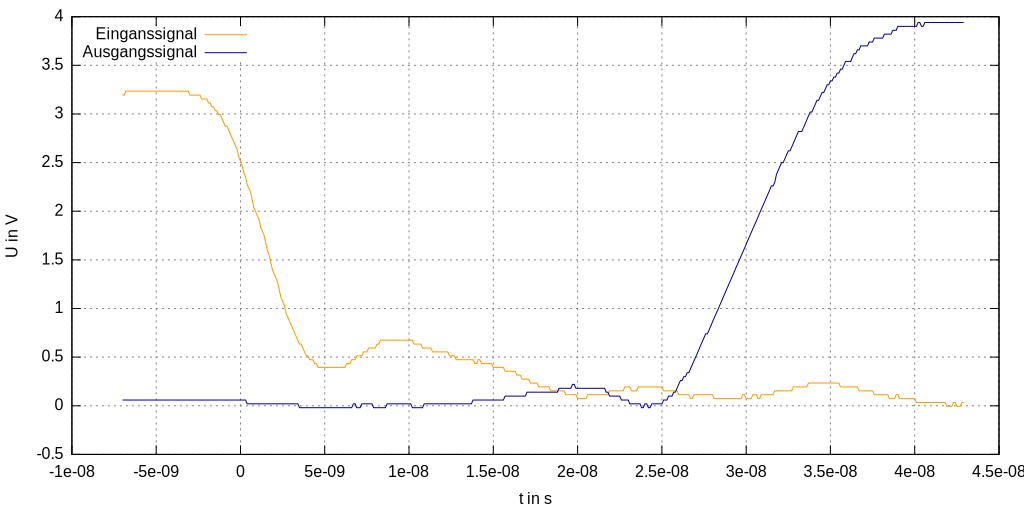
\includegraphics[width=0.8\textwidth]{komb1.pdf}
\caption{Gleichheitstest; $U\ix{e}=H\rightarrow L$}
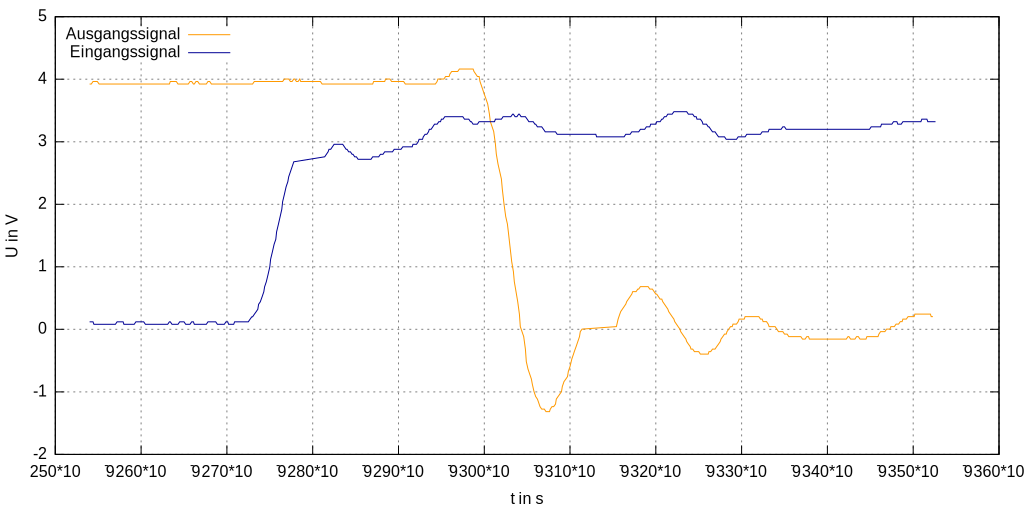
\includegraphics[width=0.8\textwidth]{komb2.pdf}
\end{figure}
Für den Übergang $U\ix{e}=H\rightarrow L$ liegt das Ergebnis des Gleichheitstests nach
\begin{align*}
 \tau\ix{G}=t_2-t_1=\unit[\left(30,8495-0.88482\right)]{\cdot 10^{-9}s}=\unit[29,964]{ns}
\end{align*}
vor. Für den Fall $U\ix{e}=L\rightarrow H$ folgt
\begin{align*}
\tau\ix{G}^{\prime}=\unit[25,837]{ns} \;
\end{align*}
Insgesamt kann man die Unschaltzeit verallgemeinern zu $T=\frac{\tau\ix{G}+\tau\ix{G}^{\prime}}{2}=\unit[27,9]{ns} \;$.
\subsubsection{Aufgabe 3}
Die Schaltung zur Siebensegmentanzeige wurde mit Hilfe eines logischen, sequentiellen Schieberegisters, wie in \ref{img:anzeigefarbe} gezeigt, aufgebaut. Selbst bei minimalem Aufwand ist die Menge der Verbindungen groß, was keine Einsicht in die Schaltvorgänge zulässt.
\begin{figure}[H]
\centering
\includegraphics[width=\textwidth]{anzeigefarb.png}
\caption{Aufbau mit getaktetem, sequentiellem Register} \label{img:anzeigefarbe}
\end{figure}
\section{Anhang}
Die originalen Messwert-Aufzeichnungen liegen bei.
\end{document}